\chapter{Testování}
Testování softwaru \cite{testing} se zaměřuje na ověření funkčnosti, spolehlivosti a~rychlosti odezvy výsledného systému. Po testu se požaduje, aby byl deterministický a~nezávislý na okolním prostředí. Test se zpravidla skládá ze tří částí. První část slouží pro přípravu prostředí pro test, nahrání testovacích dat a~vytvoření SUT (System under test). V~druhé části se volá testovaná metoda nad SUT. Třetí fáze porovnává skutečné výsledky s~těmi očekávanými. Každá technologie poskytuje vlastní knihovnu pro testování, ale tyto rysy mají společné. Existence automatických testů je nutným předpokladem pro případný budoucí refactoring. Je třeba mít na paměti, že testování nikdy nemůže sloužit jako důkaz korektnosti obdobně jako matematický důkaz. 
\newpara
V rámci testování jsou rozlišovány různé typy testů, mezi které patří akceptační, unit, integrační a~systémové testy.
\newpara
Akceptační testování vzniká ve fázi analýzy požadavků, kde jsou podle výsledné specifikace navrženy testy zaměřující se na požadavky zákazníka. Testují se jednotlivé funkcionality a~v~rámci popisu testu je zahrnut postup a~očekávaný výstup. Na základě výstupu akceptačního testování zákazník přebírá výsledný produkt.
\newpara
Unit testy píší autoři jednotlivých komponent, kde se testuje očekávané chování v~izolovaném prostředí. Při použití techniky test driven development testy vznikají před samotným kódem. V~případě, že testovaná komponenta má externí závislosti, tak závislosti dostane v~podobě namockovaných tříd. Mock je zástupná třída, která neobsahuje skutečnou implementaci, pouze si pamatuje, která metoda byla zavolána s~jakými parametry a~následně lze tyto vlastnosti ověřovat ve třetí fázi testu. K~tomu, aby bylo možné zaměnit skutečné třídy za jejich mocky, je třeba aby závislosti třídy byly předávány skrze parametry. Tato praktika se nazývá inversion of control a~bez ní nelze závislosti nahradit.
\newpara
Integrační testování je podobné unit testům, ovšem místo mockování závislostí jsou zde již použity skutečné implementace závislostí a~je testováno, zda fungují dohromady. Testuje se rozhraní mezi jednotlivými komponentami.
\newpara
Systémové testování je testování systému jako celku se všemi závislostmi. V~rámci API se testuje volání aplikačního rozhraní, návratové kódy a~vrácená data.
\newpara
Samotnou kapitolou je zátěžové testování. Zátěžové testování je metoda, která simuluje reálné podmínky a~zátěž na aplikaci za účelem zhodnocení její výkonnosti, odolnosti a~stability.


\section{Testování modelu v~rámci programu Figma}
Cílem tvorby prototypu bylo odhalit chyby v~oblasti uživatelské zkušenosti již ve fázi návrhu, a~to bez nutnosti přepisovat zdrojový kód. Iveta Brabcová společně s~vedoucím práce poskytli cennou zpětnou vazbu, která byla reflektována v následujícím návrhu.
\newpara
Samotný prototyp byl dále testován na čitelnost pro lidi s~očními vadami. Výsledek testování je uveden v~příloze \ref{appendix:simulations-of-eye-defects} Simulace očních vad pohledů prototypu v~nástroji Figma a~z~výsledků testování je patrné, že aplikace je použitelná ve všech testovaných scénářích. Testování proběhlo na pohledu hlavní strany a~prohlížeči archiválií.

\section{Testování serverové části}
Serverová část aplikace byla pokryta automatickými testy a~dodatečně testována pomocí softwaru Postman.
\newpara
V první řadě byly implementovány unit testy, které pomocí knihovny \texttt{Mockito} vytvořily zástupné závislosti. Pro jednotlivé namockované závislosti se dále definuje jejich návratová hodnota pro specifické parametry. Ve fázi ověřování výsledků se kontroluje, zda byl mock zavolán s~konkrétními parametry nebo se testuje počet zavolání dané metody.
\newpara
Integrační testy již vyžadují skutečné závislosti, a~to včetně databází. Mockito je zde použito pouze pro službu na odesílání e-mailů. Tato služba není předmětem testování. Spuštění testů vyžaduje již nasazené databáze, ovšem není žádoucí zasahovat do produkční databáze v rámci Dockeru. Systém Docker lze ovšem využít a~pomocí knihovny \texttt{TestContainer} vytvořit požadované služby pro každý test a~následně je po ukončení testu smazat. Alternativní řešení je použití relační databáze H2, která běží v~operační paměti. Toto řešení naráží na dva problémy. Navrhovaná aplikace obsahuje specifické dotazy, jež nejsou přenositelné z MariaDB do H2 a pro databázi ElasticSearch nebyla nalezena ekvivalentní in-memory databáze. Použití Docker kontejnerů značně prodlužuje dobu běhu testů a~není vhodné testy spouštět před každým přeložením aplikace. Pro testování se využívá alternativní konfigurace, která se nastavuje pomocí anotace \texttt{TestPropertySource}.
\newpara
Systémové testy již testují aplikaci jako celek. Obdobně jako u integračních testů je zde využito knihovny \texttt{TestContainer}. K~aplikaci se přistupuje pomocí třídy MockMvc, jež umožňuje emulovat zasílání HTTP požadavků na API bez nutnosti běhu aplikačního serveru. Ve Výsledku volání ověřujeme stavový kód, typ a~obsah dat. 
\newpage
\noindent
Celkem bylo na serverové části implementováno 93 testovacích scénářů ověřujících korektní chování aplikace.

\begin{figure}[htbp]
    \centering
        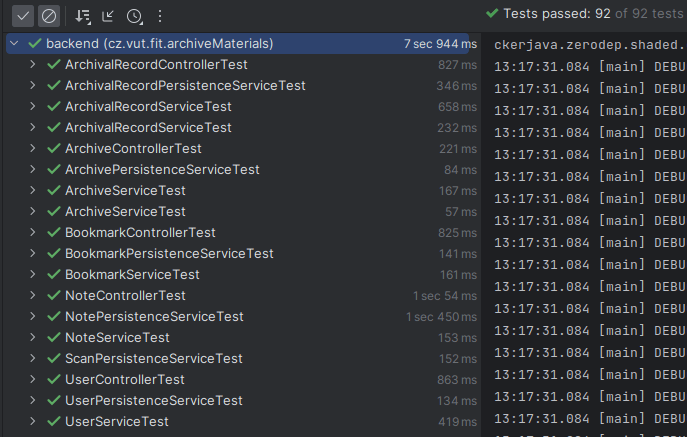
\includegraphics[scale=.6]{obrazky-figures/testing/backendTestResult.png}
        \caption{Výsledky automatických testů}
\end{figure}

\noindent
Postman umožňuje posílat HTTP požadavky včetně nastavení hlaviček. Této skutečnosti bylo využito i~u~analýzy jednotlivých systémů, kde bylo nutné rozklíčovat správné URL na mediální soubory, aby byly následně funkční v~rámci knihovny OpenSeaDragon. Jednotlivé koncové body serverové části byly vyexportovány pomocí nástroje Swagger z~OpenApi specifikace.

\section{Zátěžové testování}
 K~tomu, aby nebylo nutné nabírat desítky dobrovolníků, kteří podle metodiky budou obsluhovat systém a~bude se tak testovat zátěž, bude použit specializovaný software, který se zaměřuje na vytváření zátěžových testů. Za tímto účelem bude použit open-source nástroj JMeter, jenž má ve své paletě podporu i~pro protokol HTTP, a~bude tak možné otestovat tuto aplikaci. 
\newpara
V~rámci aplikace se vytvoří testovací plán a~skupina vláken. V~rámci skupiny vláken se nastaví počet vláken (uživatelů) a~počet cyklů. V tomto testovacím případě je zvoleno 100 uživatelů a~50 opakování scénáře. Kdyby test trval příliš krátkou dobu, tak by výsledky nemusely být přesné. 
\newpara
JMeter má podporu pro nahrávání sekvencí dotazů, takže stačí zapnout JMeter, provádět operace v~testovaném systému a~testovací plán se vytvoří automaticky. K~tomu, aby software mohl vytvořit tento plán, tak musí být v~rámci webového prohlížeče nastavena proxy skrze server JMeteru, přes který zaznamenává dotazy na konkrétní doménu. Fungování proxy bylo popsáno v~kapitole \ref{chap:implementation} Implementace. Vytvořený testovací plán obsahuje 49 volání API a~provádí se standardní úkony jako procházení stránek vyhledávání, filtrování, zobrazování detailů záznamů a~samotných snímků. JMeter je kromě samotného měření schopen získané výsledky i~vizualizovat.

\subsection{Zátěžové testování na serveru Perun}
Perun běží v~rámci školní infrastruktury a~jedná se o~první server, na který byla aplikace nasazena. 
\newpara
Server Perun je osazen šestijádrovým (dvanáctivláknovým) procesorem Intel® Xeon® E5-2630 v2. Procesor disponuje základní taktovací frekvencí 2.60 GHz a~v~turbu dosahuje taktu až 3.10 GHz. Systém je dále vybaven 16GB operační pamětí a~4GB na oddílu swap. O~spojení s~internetem se stará rozhraní od Intelu s~přenosovou rychlostí 1GBit/s.
\newpara
V průběhu testování bylo kontrolováno zatížení serveru, které oscilovalo mezi 80-90 \%. Zatížení serveru bylo kontrolováno pomocí programu Htop a~podle vytížení jader aplikace rovnoměrně distribuuje úlohy.

\begin{figure}[htbp]
    \centering
        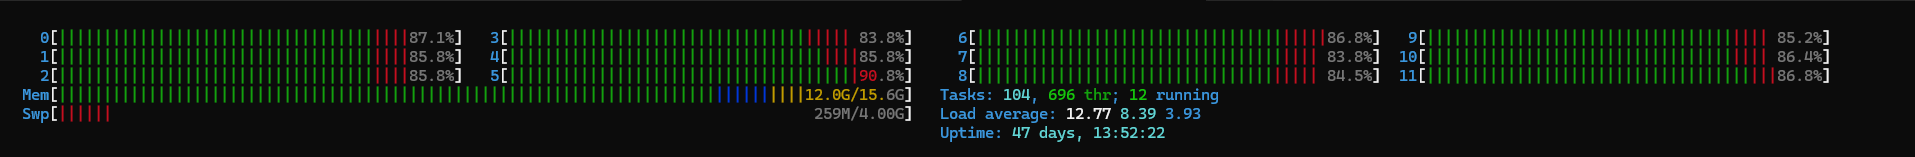
\includegraphics[scale=.2]{obrazky-figures/testing/performance/perun/htop.png}
        \caption{Zatížení serveru Perun v průběhu testu}
\end{figure}

\noindent
V průběhu testu, který trval 15 minut, bylo zasláno 245 000 požadavků. Z~tohoto necelého čtvrt milionu požadavků žádný neskončil chybou, což značí, že systém tuto zátěž ustál.
\newpara
Jak je vidět na grafu \ref{fig:average-response-perun}, tak průměrná doba odezvy se pohybovala okolo 500 ms. Akceptovatelná mez u~informačních systémů se pohybuje do 2s \cite{performanceLatency}. 
\begin{figure}[htbp]
    \centering
        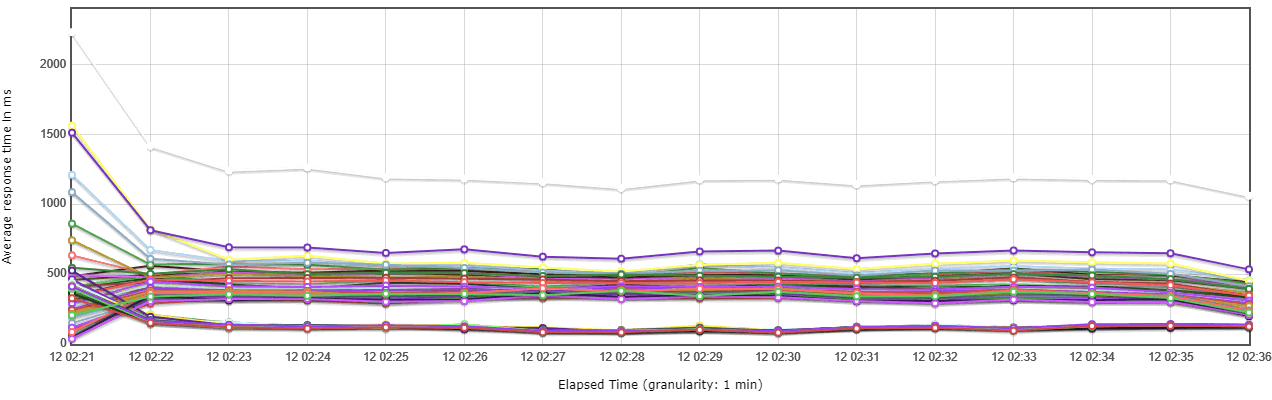
\includegraphics[scale=.34]{obrazky-figures/testing/performance/perun/flotResponseTimesOverTime.png}
        \caption{Průměrná doba odpovědi}
        \label{fig:average-response-perun}
\end{figure}

\newpage
\noindent
Na grafu \ref{fig:percentil-response-perun} jsou vidět jednotlivé percentily, kde oranžová horní spojnice značí maximum a~fialová spojnice medián. Zajímavější údaj než maximum je zelená spojnice, která značí percentil 99. Žlutá spojnice dále reprezentuje percentil 95 a~dolní červená spojnice percentil 90. To znamená, že již u~percentilu 99 je většina dotazů pod 2 vteřiny.

\begin{figure}[htbp]
    \centering
        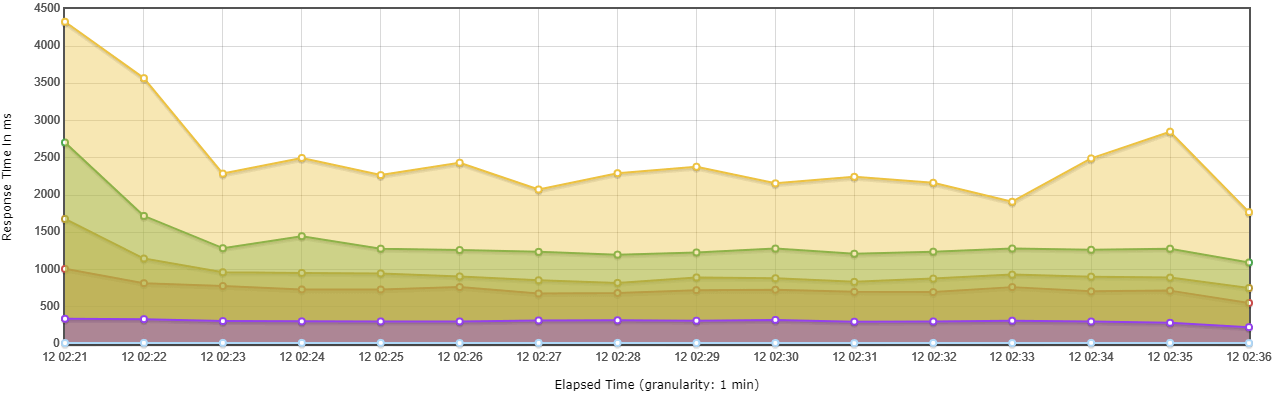
\includegraphics[scale=.34]{obrazky-figures/testing/performance/perun/flotResponseTimePercentilesOverTime.png}
        \caption{Percentil průměrné doby odpovědi}
        \label{fig:percentil-response-perun}
\end{figure}

\noindent
Zde je porovnání odezvy rozděleno do tří kategorií, přičemž dle zvoleného kritéria jsou přípustné zelené a~žluté hodnoty.

\begin{figure}[htbp]
    \centering
        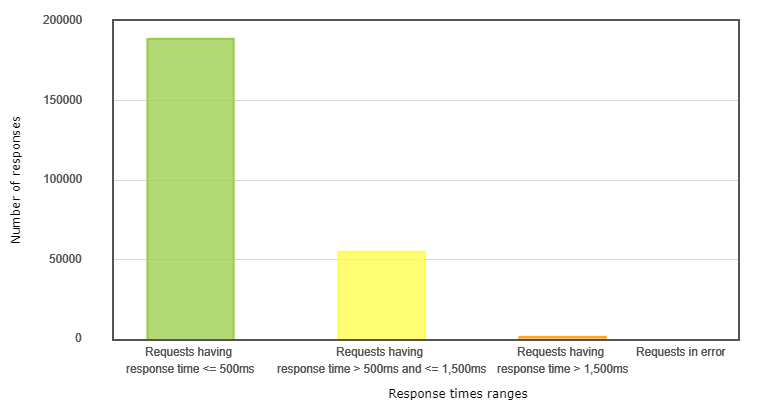
\includegraphics[scale=.55]{obrazky-figures/testing/performance/perun/responseTimeOverview.png}
        \caption{Přehled latence}
\end{figure}
\newpage
\noindent
V průběhu testu bylo odesláno ze serveru více než 2MB dat každou vteřinu. 
\begin{figure}[htbp]
    \centering
        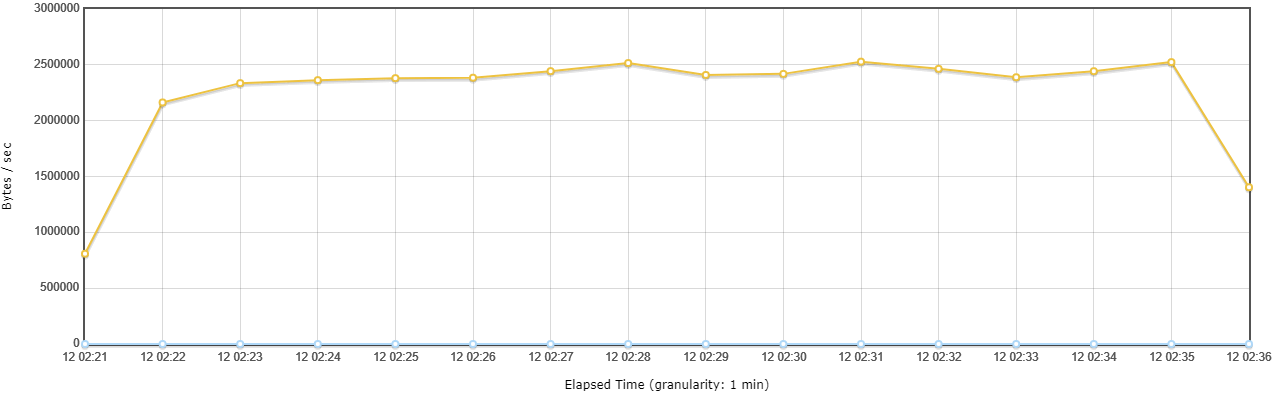
\includegraphics[scale=.34]{obrazky-figures/testing/performance/perun/flotBytesThroughputOverTime.png}
        \caption{Datová propustnost}
\end{figure}

\subsection{Zátěžové testování na serveru Radegast}
Radegast běží v~rámci školní infrastruktury a~jedná se o~server, na který má být aplikace v~budoucnu přesunuta. Za tímto účelem byl vznesen požadavek vedoucím práce na porovnání výkonosti serverů Radegast a Perun.
\newpara
Server Radegast je osazen modernějším šestnáctijádrovým (třicetidvouvláknovým) procesorem EPYC 7313 od konkurenční značky AMD. Procesor za cenu skoro dvojnásobného TDP nabízí základní takt 3.0GHz a~v~turbo režimu dokonce 3.7GHz. Velikost operační paměti zde činí 66GB, což je čtyřnásobný nárůst oproti serveru Perun. Server dále disponuje dvěma síťovými kartami. Pomalejší karta disponuje přenosovou rychlostí 1GBit/s a~druhá rychlostí 10GBit/s.
\newpara
V~průběhu testování bylo kontrolováno zatížení serveru, které oscilovalo okolo 40~\%, což je výrazné zlepšení oproti serveru Perun.
Zatížení serveru bylo kontrolováno pomocí programu Htop a~podle vytížení jader aplikace 
rovnoměrně distribuuje úlohy.

\begin{figure}[htbp]
    \centering
        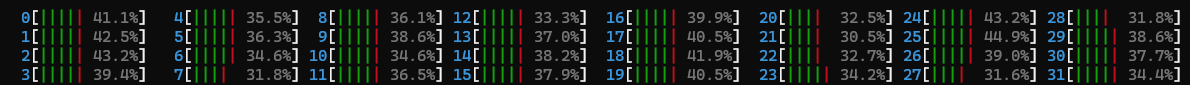
\includegraphics[scale=.35]{obrazky-figures/testing/performance/radegast/htop.png}
        \caption{Zatížení serveru Radegast v průběhu testu}
\end{figure}

\noindent
Test i~jeho parametry jsou shodné s~testováním serveru Perun. Test trval kratší dobu a~v~průběhu se vyskytlo několik chyb. Všechny chyby vznikly na proxy serveru, takže s~velkou pravděpodobností archivní web nevrátil včas odpověď. 
\newpage
\noindent
Jak je vidět na grafu \ref{fig:average-response-radegast}, tak průměrná doba odezvy se pohybovala okolo 150 ms, což je výrazné zlepšení oproti předchozímu serveru.
\begin{figure}[htbp]
    \centering
        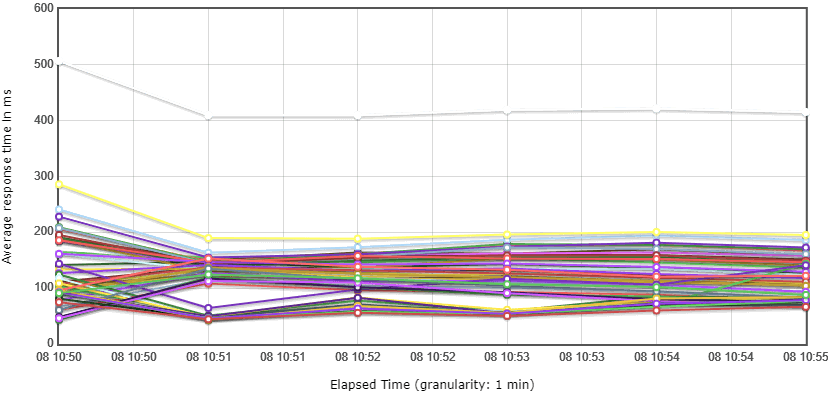
\includegraphics[scale=.5]{obrazky-figures/testing/performance/radegast/flotResponseTimesOverTime.png}
        \caption{Průměrná doba odpovědi}
        \label{fig:average-response-radegast}
\end{figure}

\noindent
Na grafu \ref{fig:percentil-response-radegast} jsou vidět jednotlivé percentily, kde oranžová horní spojnice značí maximum a~fialová spojnice medián. Zajímavější údaj než maximum je zelená spojnice značící percentil 99. Žlutá spojnice dále reprezentuje percentil 95 a~dolní červená spojnice percentil 90. To znamená, že již u~percentilu 99 jsou dotazy okolo 500 ms, což je hluboko pod hranicí 2~vteřin.

\begin{figure}[htbp]
    \centering
        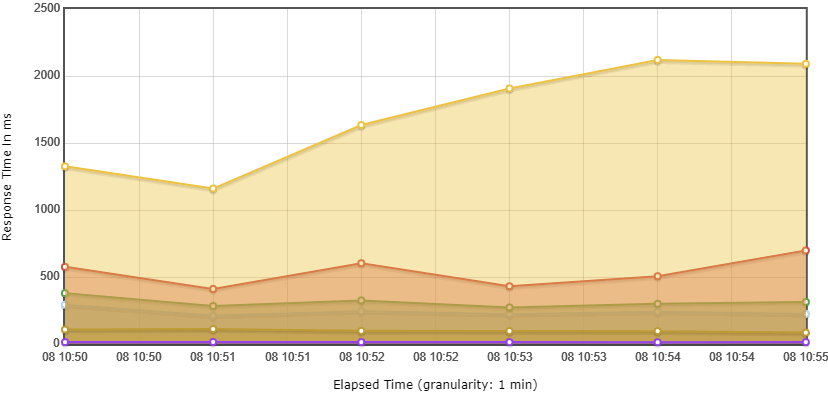
\includegraphics[scale=.5]{obrazky-figures/testing/performance/radegast/flotResponseTimePercentilesOverTime.png}
        \caption{Percentil průměrné doby odpovědi}
        \label{fig:percentil-response-radegast}
\end{figure}
\newpage
\noindent
Zde je porovnání odezvy rozděleno do tří kategorií, přičemž dle zvoleného kritéria jsou přípustné zelené a~žluté hodnoty.

\begin{figure}[htbp]
    \centering
        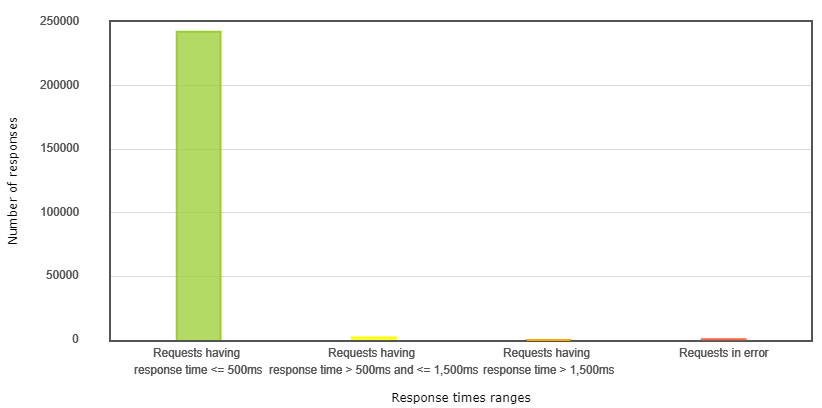
\includegraphics[scale=.5]{obrazky-figures/testing/performance/radegast/responseTimeOverview.png}
        \caption{Přehled latence}
\end{figure}
\noindent
V~průběhu testu bylo odesláno ze serveru okolo 6MB dat každou vteřinu. 
\begin{figure}[htbp]
    \centering
        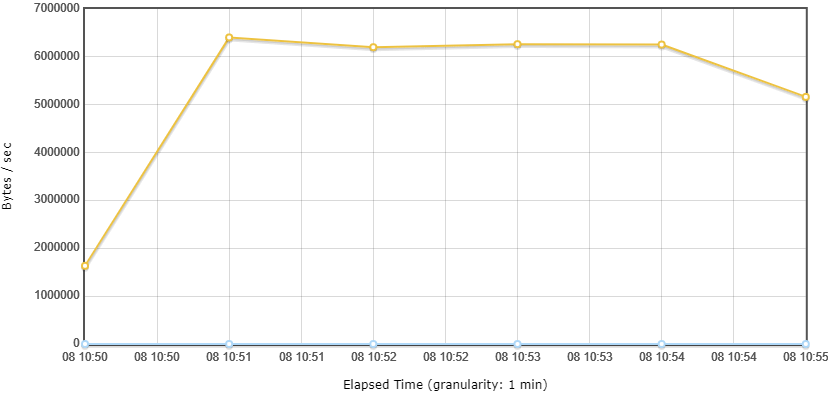
\includegraphics[scale=.5]{obrazky-figures/testing/performance/radegast/flotBytesThroughputOverTime.png}
        \caption{Datová propustnost}
\end{figure}

\subsection{Výsledky porovnání}
Ze zmíněných grafů je patrné, že server Radegast je výrazně rychlejší než server Perun, což je očekávatelné vzhledem k~novějšímu hardwaru, kde například procesor je o~osm let mladší než u serveru Perun. Průměrná doba odezvy spadla z~500 ms na 150 ms, což se kladně projeví při simultánním přístupu více uživatelů.

\section{Testování odbornou veřejností}
Systém byl po nasazení prezentován odborné veřejnosti skrze soukromou skupinu \\\texttt{Genealogie CZ+SK} na sociální síti Facebook. Příspěvek nasbíral přes 80 reakcí a~60 komentářů.
Mnoho komentářů se věnovalo problematice rozšíření datových sad aplikace. Několik uživatelů se podělilo o~uživatelskou zkušenost s~nově vyvíjeným systémem. Došlo přibližně k~patnácti úpravám v~oblasti uživatelské zkušenosti na základě zpětné vazby od uživatelů.